\subsection{The Operation}

This paragraph is branched into three sections, before the beginning of the game, the game start, and the end of the game. 

\subsubsection{Before beginning of the game}
When the game is activated, a primary window is created and appeared, but the current interface cannot be clicked or manipulated by any action. Therefore, there are a few steps that can begin and activate a new game, which is shown below: 

\begin{enumerate}
	\item\textbf{The menu item "New Game"}\\
	The user should press the Menu Item "New Game" on the top-left corner to generate a new game.
	
	\item\textbf{Number of participants}\\
	Since the new game has been generated, a secondary scene which is for initiating player state arises. On the top-left corner of this secondary scene, the user can select the check menu Item to determine how many players should exist in a game. 
	
	\item\textbf{Inserting participants name and status}\\
    According to the selection of the number of participants, the user can insert every participant's name and decide which player is a bot or human.
	
	\item\textbf{Apply}\\
	At last, press the button, which is on the bottom-right corner to execute the game.
	
\end{enumerate}

\subsubsection{Game start}

\begin{enumerate}
	\item\textbf{A player's turn}\\
    During the game playing, one of the designs should be noticed that the game is being operated based on the turn of the current player. The hand token can be manipulated for the current player, nevertheless, other hand tokens are not allowed to give any movement or action.
	
	\item\textbf{Utilising tokens}\\
	Here have two different manipulative approaches for symbol tokens and action tokens. The instruction for two types of tokens is below:
	\begin{itemize}
		\item{Symbol token} \\
	    The manipulation behaviour of the symbol token is using drag and drop. The user needs to move their mouse on the symbol token of his or her hand token, which is chosen to move. And hold the left click and drag it to the chess board and release it on the desired cell of the chess board.  
		
		\item{Action token} \\
		The manipulative approach for using action tokens is clicking. Four action tokens use clicking action to activate the function of the action token. Firstly, as the user decides to use the action token, which is in his or her hand, it is simply a single click on the action token. However, the important and necessary noticed gist is that once the action token has been clicked, the user is not allowed to have other tokens chosen.  
		
		\begin{itemize}
			\item{Remove} \\
			The user should directly click on the desired cell of the chess board. Indeed, it is vital to realize that Remove is only allowing to click on the cell which has already occupied a token.  
			
			\item{Shifting} \\
	    	Based on the instruction of the shifting function, the user should select two positions on the board after clicking on the shifting token on their token hand. One is the position that contains a symbol token on a cell of the chess board and another should be an empty position which means no symbol token is placed.  
			
			\item{Exchange} \\
		    Regarding the function of the exchange token, the user has to choose two tokens on the chess board. After two tokens are selected by clicking, the animation of exchanging tokens is shown up to swap these two chosen tokens.  
			
			\item{Replace} \\
			Replace token has a unique function among these four action tokens. As the replace token has been activated, the user needs to select one symbol token on his or her hand before choosing another board token, which will be replaced.  
			Hence, if there is no other symbol token on the player's hand, then the Replace token cannot be executed.
			
		\end{itemize}
		
		
	\end{itemize}
	
	\item\textbf{Highlighting tokens}\\
	One design for raising up the game experience for players is that highlight every token, which is being dropped, clicked, or swapped. 
	Indeed, the token can be immediately and apparently noticed by highlighting after they are being changed position. 
	
\end{enumerate}

\newpage
\subsubsection{End the game}
Along with the game approaching the end and the winner is determined and appears, an alert message has emerged with a window like a Figure \ref{fig:winnerMessage} below. The message shows which team is winning the game and also the reason for winning the game.  

However, once the message is read and closed, the main interface becomes disabled to access or manipulate until the user selects a new game on the menu item.  

\begin{figure}[h]
	\centering
	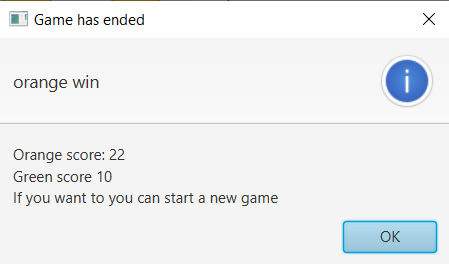
\includegraphics[width=0.5\textwidth]{image/winner message}
	\caption{The winning message}
	\label{fig:winnerMessage}
\end{figure}

